%%%%%%%%%%%%%%%%%%%%%%%%%%%%%%%%%%%%%%%%%%%%%%%%%%%%%%%%%%%%%%%%%%%
%%% Documento LaTeX 											%%%
%%%%%%%%%%%%%%%%%%%%%%%%%%%%%%%%%%%%%%%%%%%%%%%%%%%%%%%%%%%%%%%%%%%
% Título:	Plantilla de TFG
% Autor:  Carlos Andres Goez, Juan Pablo Baena 
% Fecha:  2020-03-12
%%%%%%%%%%%%%%%%%%%%%%%%%%%%%%%%%%%%%%%%%%%%%%%%%%%%%%%%%%%%%%%%%%%
%	Modo:					PDFLaTeX.
%%%%%%%%%%%%%%%%%%%%%%%%%%%%%%%%%%%%%%%%%%%%%%%%%%%%%%%%%%%%%%%%%%%
%-----------------------------------------------------------------%
% Clase de documento: libro
\documentclass[10pt,a4paper]{book} % article, report, book.

% Preámbulo: paquetes, comandos, entornos, estilos y título de página.
%%%%%%%%%%%%%%%%%%%%%%%%%%%%%%%%%%%%%%%%%%%%%%%%%%%%%%%%%%%%%%%%%%%
%%% Documento LaTeX 											%%%
%%%%%%%%%%%%%%%%%%%%%%%%%%%%%%%%%%%%%%%%%%%%%%%%%%%%%%%%%%%%%%%%%%%
% Título:	Plantilla de TFG/TFM
% Autor:  Carlos Andres Goez, Juan Pablo Baena 
% Fecha:  2020-03-12
%%%%%%%%%%%%%%%%%%%%%%%%%%%%%%%%%%%%%%%%%%%%%%%%%%%%%%%%%%%%%%%%%%%
%	Modo:					PDFLaTeX.
%%%%%%%%%%%%%%%%%%%%%%%%%%%%%%%%%%%%%%%%%%%%%%%%%%%%%%%%%%%%%%%%%%%
%------------------------------

%1 Codificación e idioma%
\usepackage[utf8]{inputenc} %Codificación en latin-1%
\usepackage[T1]{fontenc} %Codificación de fuente%
\usepackage[spanish, es-tabla]{babel}	%Hyphenation (Guionado) en español%
\usepackage{eurosym} % Tipografia
%2 Matemáticas y Física %
% Importante para ecuaciones, magnitudes y unidades%
\usepackage{amssymb,amsmath,latexsym,amsfonts} % paquetes estándar%
\usepackage{ifthen} %sentencias if y while%
%3 Gráficos%
\usepackage{graphics,graphicx,subcaption} %paquetes gráficos estándar%
%\usepackage{subfigure} %permite varias subfiguras en una figura
\usepackage{wrapfig} %paquete para gráfica lateral%
\usepackage{float} %figuras flotantes%
% \begin{floatingfigure}[r]/[l]{4.5cm}
% \end{floatingfigure}
\usepackage{graphpap}	%comando \graphpaper en el entorno picture%

%4 Estilo y formato%
\usepackage{imakeidx} %MakeIndex%
%Comando para crear glosario (index en inglés)
\makeindex[columns=2, title=Glosario, intoc]
%\usepackage{showidx} % Hace que cada comando \index se imprima en la página donde se ha puesto (útil para corregir los índices)
\usepackage{fancyhdr}	%cabeceras y pies mejor que con \pagestyle{}%
\setlength{\headheight}{16pt}% ...at least 16pt
\usepackage{titlesec,titletoc} %Formateo de secciones y títulos%
\raggedbottom %Para fragmentar versos en varias páginas%
\usepackage{alltt} % Define el environment alltt, como verbatim, excepto que \, { y } tienen su significado normal. Se describe en el fichero alltt.dtx.
\usepackage[pdftex,bookmarksnumbered,hidelinks]{hyperref} %hyper-references%
\usepackage{minitoc} % Para poner tablas de contenido en cada capítulo.
\usepackage{listings} % Para escribir piezas de código C, Python, etc. %
%listings configuration
\lstset{
	language=Python, %Puede ser C, C++, Java, etc.
	showstringspaces=false,
	formfeed=\newpage,
	tabsize=4,
	commentstyle=\itshape,
	basicstyle=\footnotesize\ttfamily,
	escapeinside={(@}{@)},
	morekeywords={models, lambda, forms}
}
\renewcommand{\lstlistingname}{Listado}

\usepackage{tipa} % tipografía IPA (International Phonetic Alphabet)
\usepackage{longtable} %Entorno Longtable, fracciona tablas a lo largo de páginas%
\usepackage{xcolor}
\usepackage{colortbl}
\usepackage{emptypage} %Para eliminar el número de página en páginas sin contenido (\cleardoublepage)
%%%%%%%%%%%%%%%%%%%%%%%%%%%%%%%%%%%%%%%%%%%%%%%%%%%%%%%%%%%%%%%%%%%
%%% Documento LaTeX 											%%%
%%%%%%%%%%%%%%%%%%%%%%%%%%%%%%%%%%%%%%%%%%%%%%%%%%%%%%%%%%%%%%%%%%%
% Título:	Plantilla de TFG/TFM
% Autor:  Carlos Andres Goez, Juan Pablo Baena 
% Fecha:  2020-03-12
%%%%%%%%%%%%%%%%%%%%%%%%%%%%%%%%%%%%%%%%%%%%%%%%%%%%%%%%%%%%%%%%%%%
%	Modo:					PDFLaTeX.
%%%%%%%%%%%%%%%%%%%%%%%%%%%%%%%%%%%%%%%%%%%%%%%%%%%%%%%%%%%%%%%%%%%
%------------------------------
\newcommand{\tfgtitlename}{	SISTEMA SEMIAUTOMÁTICO PARA CLASIFICACIÓN, EMPAQUE Y MONITOREO EN POSTCOSECHA DE HORTENSIAS}
\newcommand{\tfgtitlenameENG}{<Título del TFG en inglés>}
\newcommand{\tfgauthorname}{Carlos Andrès Góez Aguirre\\ Juan Pablo Baena Martìnez}
\newcommand{\tfgtutorname}{Edgar Virgilio}
\newcommand{\tfganno}{2020}
\newcommand{\tfgUniversidad}{Universidad EIA}
\newcommand{\tfgCiudad}{Envigado}
\newcommand{\tfgCarrera}{Ingeniería Mecatrónica}

% 2 Comandos a nivel de texto %
\newcommand{\R}{\textsuperscript{\textregistered}}	%Símbolo registrado%
\newcommand{\C}{\textsuperscript{\copyright}}	%Símbolo Copyright%
\newcommand{\TM}{\texttrademark} %Símbolo Trade Mark (marca comercial)%

% 2.1 Comandos abreviatura %
\newcommand{\tit}{\textit} %Fuente cursiva (itálica)%
\newcommand{\tbf}{\textbf} %Fuente negrita%
\newcommand{\ttw}[1]{\texttt{#1}} %Fuente máquina de escribir (typewriter)%
%Combinación%
\newcommand{\textittt}[1]{\textit{\texttt{#1}}} %itálica y typewriter%
\newcommand{\textittw}{\textittt} % Otra forma de escribirlo.
\newcommand{\tittw}{\textittw} %Shortened%
\newcommand{\tbftw}[1]{\tbf{\ttw{#1}}}

%Crea una nueva línea y la indenta sin crear interlineado extra.
\newcommand{\nli}{\\ \indent}

%Para escribir un correo electrónico%
\newcommand{\mailto}[1]{\href{mailto:#1}{#1}}

% Si vas a hacer un uso básico de \index (entradas en el índice de sólo un nivel, sin formatos especiales, etc.), define la orden
\newcommand{\miindex}[1]{#1\index{#1}}

\newcommand{\hs}{\hspace} % Abreviatura espacio horizontal
\newcommand{\vs}{\vspace} % Abreviatura espacio vertical

% Abreviaturas para los conjuntos de números más comunes.
\newcommand{\realnumbers}{\mathbb R}
\newcommand{\naturalnumbers}{\mathbb N}
\newcommand{\integernumbers}{\mathbb Z}
\newcommand{\rationalnumbers}{\mathbb Q}
\newcommand{\complexnumbers}{\mathbb R}
\newcommand{\irrationalnumbers}{\mathbb I}

% Doble barra sobre una letra (para expresar las matrices).
\newcommand{\doublebar}[1]{\bar{\bar{#1}}}
% Ej: \vector(y) = \doublebar(A) \vector(x) (Stma. lineal de ec.)

% 3 Comandos a nivel de entorno %
\newcommand{\benu}{\begin{enu}} % Begin enumerate
	\newcommand{\eenu}{\end{enu}} 	% End enumeration

%Comando para escribir código Python
\newcommand{\code}[3]{
	\begin{minipage}{0.96\linewidth}
		\begin{center}
			\lstinputlisting[
			language   = Python,
			frame      = lines,
			framexleftmargin = 5mm,
			caption    = {#1},
			label      = {#3},
			]{#2}
		\end{center}
	\end{minipage}
}

% 4 Comandos a nivel de página y sección %
%Crea página en blanco
\newcommand{\blankpage}{\clearpage{\pagestyle{empty}\cleardoublepage}}

% Versión x del comando section: sin numeración pero sí aparece en la tabla de contenidos.
\newcommand{\sectionx}[1]{
	\section*{#1}
	\addcontentsline{toc}{section}{#1}
}

% Versión y del comando section: sin numeración y NO aparece en la tabla de contenidos.Ignacio Moreno Doblas
\newcommand{\sectiony}[1]{
	\section*{#1}
}

% Versión x del comando chapter: sin numeración pero sí  aparece en la tabla de contenidos.
\newcommand{\chapterx}[1]{
	\chapter*{#1}
	%\addcontentsline{toc}{chapter}{#1} %Caused by minitoc package%
	\addstarredchapter{#1} %For minitoc package%
}

% substituto del comando \chapter: incluye estilo de página.
\newcommand{\chapterbegin}[1]%
{%
	\pagestyle{fancy}
	\renewcommand{\headrulewidth}{1pt}
	\fancyhead[LE,RO]{\thepage}
	\fancyhead[RE]{Capítulo \thechapter. #1}
	%\fancyhead[RE]{Parte \thepart \rightmark} %
	\fancyhead[LO]{\nouppercase{\rightmark}} %
	\fancyfoot[CE,CO]{} %
	
	\chapter{#1}
}

% Versión x del comando \chapterbegin: sin numeración y aparece en la tabla de contenidos.
\newcommand{\chapterbeginx}[1]%
{%
	\pagestyle{fancy}
	\renewcommand{\headrulewidth}{1pt}
	\fancyhead[RO,LE]{\thepage}
	\fancyhead[RE,LO]{#1}
	%\fancyhead[LO]{Chapter \thechapter}
	%\fancyhead[RE]{Part \thepart} %
	\fancyfoot[CE,CO]{} %
	
	\chapterx{#1}
}

%Fin de capítulo
\newcommand{\chapterend}{
	\cleardoublepage 
	\thispagestyle{empty}
}
%Si fuera un artículo en lugar un libro, \clearpage en lugar de \cleardoublepage

% 5 Otros comandos %
%\let\Oldpart\part
%\newcommand{\parttitle}{}
%\renewcommand{part}[1]{\Oldpart{#1}\renewcommand{\parttitle}{#1}} %Header customization%

%Cambiar el título índice de capítulo a ``Contenido''.
\renewcommand{\mtctitle}{Contenido}

\dominitoc % Para tablas de contenidos por capítulo.

\addto{\captionsspanish}{
	\renewcommand{\listtablename}{Índice de Tablas}
	\renewcommand{\tablename}{Tabla} } % Por ejemplo, modificar el nombre de 'Cuadro' a 'Tabla'.

\addto{\captionsspanish}{
	\renewcommand{\contentsname}{Índice} }

% Si se desea cambiar el tipo de letra a Computer Modern
% por cualquier razón, comenta las siguientes
% dos líneas
\renewcommand{\rmdefault}{phv} % Arial
\renewcommand{\sfdefault}{phv} % Arial

%\addto{\captionsspanish}{
%	\renewcommand{\partname}{Fase} }

%\addto{\captionsspanish}{%
%    \renewcommand{\refname}{\vspace{-4.5ex}}} % Para que no aparezca el texto 'referencias' en la bibliografía.

% Modifica el interlineado
%\renewcommand{\baselinestretch}{1.5}

% Definición de longitudes para usar en los entornos:
%
% Normal parskip.
\newlength{\parskipenv}
\setlength{\parskipenv}{\parskip}

\newlength{\parindentenv}
\setlength{\parindentenv}{\parindent}
%%%%%%%%%%%%%%%%%%%%%%%

% 1 dobleindent
%El entorno dobleindent está pensando para escribir párrafos con doble indentación a cada lado.
%Tiene dos parámetros de entrada con las distancias medidas desde los márgenes de página.

\newenvironment{dobleindent}[2]
	%Comienzo de nuevo entorno%
	{
	\begin{list}
		{}
		{
		% Left and right margins:
		\leftmargin = #1
		\rightmargin = #2
		%
		% Separation from preceding and following text:
		\topsep = 0ex
		\partopsep = 0ex
		\parsep = \parskipenv
		%
		% Indentation for paragraphs:
		\itemsep = \parskipenv
		\itemindent = \parindentenv
		\listparindent = \itemindent
		%
		% Horizontal separation from label:
		\labelsep = 1ex
		\settowidth{\labelwidth}{0cm}
		}

		 \item}
	% End new env
	{\end{list}}

%%%%%%%%%%%%%%%%%%%%%%%%%%%%%
%2 izqindent
% El entorno izqindent sólo crea un párrafo indentado a la izquierda.
\newenvironment{izqindent}[1]
{
\begin{dobleindent}{#1}{0cm}
}
{
\end{dobleindent}
}

%%%%%%%%%%%%%%%%%%%%%%%%%%%%%
% 3 dobleindentx
% El entorno dobleindentx es una variación del dobleindent usando leftskip y rightskip.
% Aunque es más limitado, también se puede usar.
\newenvironment{dobleindentx}[2] % Sólo funciona en modo paragraph
{ % Preamble
  \leftskip = #1
  \rightskip = #2
}
{ % Postamble
\leftskip = 0cm
\rightskip = 0cm
}

%%%%%%%%%%%%%%%%%%%%%%%%%%%%%
% 4 ite
% El entorno ite es una modificación del entorno itemize estándar de \LaTeX. Puede usarse o modificarse si el usuario lo desea.
% También puede parametrizarse el entorno enumerate o description de forma equivalente.
\newenvironment{ite}
	{
		\begin{izqindent}{\parindent}
		\hspace{-\parindent} 	% compensación del sangrado que introduce el entorno.
		\vspace{-1.0\parskip}	% compensación del \parskip que introduce el entorno.
		\vspace{-\baselineskip}	% compensación por la línea que introduce el entorno.
		\begin{itemize}
	}
	{
		\end{itemize}
		\end{izqindent}
	}

%%%%%%%%%%%%%%%%%%%%%5
% commando stdformat para formatear los entornos descript, enu y itemization.
\newcommand{\stdformat}
	{% Declarations for format presentation.
		%
		% Separation from preceding and following text:
		\setlength{\topsep}{1ex}%
		\setlength{\partopsep}{0ex} %
		%
		% Horizontal separation from label:
		\labelsep = 1ex
		\setlength{\labelwidth}{0ex}
		%
		%	Left and right margins:
		\setlength{\leftmargin}{1cm}%
		\addtolength{\leftmargin}{\labelsep}
		\setlength{\rightmargin}{0ex}
		%
		% Indentation for paragraphs:
		\setlength{\itemindent}{-\leftmargin}%
		\addtolength{\itemindent}{1ex}
		\setlength{\listparindent}{\parindent}%
		%
		% Separation between paragraphs.
		\setlength{\parsep}{\parskipenv}%
		\setlength{\itemsep}{1ex}
	}

%%%%%%%%%%%%%%%%%%%%%%%%%%%%%
% 5 descript

\newenvironment{descript}
	% Beginning new env def.
	{
		\begin{list}
			{} % No default label for \item.
			{
				% Declarations for format presentation.
				\stdformat
				%
				\renewcommand{\makelabel}[1]{\normalfont\bfseries##1\hfil}
			}
	}
	% Ending new env def.
	{
		\hspace*{\fill} \\ \end{list}
	} % Se introduce un salto de línea para que el texto siguiente esté separado.
%END newenvironment{descript}

%%%%%%%%%%%%%%%%%%%%%%%%%%%%%
% 6 enu
\newcounter{itemnumber} % Counter for the environment.

\newenvironment{enu}
	% Beginning new env def.
	{
		\begin{list}
		{
			\raggedleft \arabic{itemnumber}
		}
		{
			\usecounter{itemnumber}
			\stdformat
		}
	}
	{
		\end{list}
	}

%%%%%%%%%%%%%%%%%%%%%%%%%%%%%
% 7 itemization
\newenvironment{itemization}
	% Beginning new env def.
	{
		\begin{list}
			{$\bullet$} % No default label for \item.
			{
				% Declarations for format presentation.
				\stdformat
			}
	}
	% Ending new env def.
	{
		\end{list}
	}


%%%%%%%%%%%%%%%%%%%%%%%%%%%%%
% 8 sinopsis
\newenvironment{sinopsis}{%[1]{
	\sectiony{Sinopsis}
	%\label{#1}
} {
%	\pagebreak
}

% Tabla de materias:
%--------------------%
% 1 Márgenes de página
%%%%%%%%%%%%%%%%%%%%%%%
% Para conocer los parámetros de diseño de páginas, tales como
%  los márgenes izquierdo, derecho, anchura de página, etc.
%  véase el archivo ``Page layout.png'' que acompaña esta plantilla.
% Así se conocerá mejor cómo adaptar el documento según los
%  requisitos del usuario.

% 1 Márgenes de página
%-------------------------------%
% Parámetros de estilo de página.
% DIN A4: 29.7 cm x 21 cm
%		área neta: 3 cm + 3 cm + 15 cm.
%
% Definición de márgenes de página
%  even para páginas pares
%  odd  para páginas impares
\newlength{\realoddsidemargin}	  % \oddsidemargin menos 1 in.
\newlength{\realevensidemargin}		% \evensidemargin menos 1 in.
\newlength{\realtopmargin}				% \topmargin menos 1 in.
%
% Asignación de márgenes de página
% ASIGNESE en caso de querer cambiarlo
\setlength{\realtopmargin}{2cm}			% REAL top margin.
\setlength{\realoddsidemargin}{3cm}		% REAL oddside margin.
\setlength{\realevensidemargin}{3cm}	% REAL evenside margin.
\setlength{\hoffset}{0cm}
\setlength{\voffset}{0cm}
%
% Substracción de 1 pulgada de compensación
%  (véase ``Page Layout.png'' para más información)
\addtolength{\realoddsidemargin}{-1in}	% 1 inch = 2.54 cm.
\addtolength{\realevensidemargin}{-1in}
\addtolength{\realtopmargin}{-1in}
%
% Asignación de anchuras y márgenes
% No hay notas al margen
\setlength{\marginparsep}{0cm} % No van a existir notas al margen
\setlength{\marginparwidth}{0cm} % No van a existir notas al margen
%
% Asignación de anchura de texto
\setlength{\textwidth}{15cm}	% Anchura neta del texto (globalmente).
%
% Asignación de márgenes par, impar y en altura
\setlength{\oddsidemargin}{\realoddsidemargin}	% odd-page left margin (global).
\setlength{\evensidemargin}{\realoddsidemargin}	% even-page left margin (global).
\setlength{\topmargin}{\realtopmargin}					% top margin (Global).

% Deja un pequeño espacio vertical entre párrafos
\setlength{\parskip}{1ex}



% Document body.
%-------------------------------------------------------------------%
\begin{document}

% Formato de documento hasta el capítulo 1 (sin incluirlo)
\frontmatter


%%% Tipos de portada %%%
%	1. \maketitle
%	2. titlepage
%%%%%%%%%%%%%%%%%%%%%%%%

%	1. \maketitle
%%%%%%%%%%%%%%%%%%%%%%%%
%\maketitle
\thispagestyle{empty}

%	2. titlepage
%%%%%%%%%%%%%%%%%%%%%%%%
%\begin{titlepage}

	\begin{center}
		\Large \scshape
		Universidad de Málaga\\
		\bigskip
		Escuela Técnica Superior de\\
		Ingeniería de Telecomunicación
	\end{center}

	\bigskip

% \begin{center}
% 	\begin{tabular}{lcr}
% 		\includegraphics[height=3cm,keepaspectratio]{figuras/MarcaETSIT.jpg} & \hspace{2cm}
% 		\includegraphics[height=2.5cm,keepaspectratio]{figuras/UnivMalacitana.pdf}
% 	\end{tabular}
% \end{center}

\bigskip

	\bigskip \bigskip \bigskip \bigskip

	\begin{center}
		\Large \scshape
		TRABAJO FIN DE GRADO
	\end{center}

	\bigskip \bigskip \bigskip \bigskip

	\begin{center}
		\huge \scshape
		\tfgtitlename %Actualizar esta variable en A2.Preambulo.comandos.tex
	\end{center}

	\vfill

	\begin{center}
		\Large \scshape
		Grado en Ingeniería de\\
		<nombre de la titulación>
	\end{center}

	\bigskip \bigskip \bigskip \bigskip
%	\vfill


%	{\large Málaga, \tfganno \hfill \tfgauthorname}
	\begin{flushright}
		\large \scshape
		\tfgauthorname \\%Actualizar esta variable en A2.Preambulo.comandos.tex
		Málaga, \tfganno %Actualizar esta variable en A2.Preambulo.comandos.tex
	\end{flushright}
	%\blankpage
%\end{titlepage}

\blankpage

% Resumen del TFG en español
%%%%%%%%%%%%%%%%%%%%%%%%%%%%%%%%%%%
% Página de resumen del proyecto %
%%%%%%%%%%%%%%%%%%%%%%%%%%%%%%%%%%
% !TEX root = Documento_TG.tex

\pagestyle{fancy}
\renewcommand{\headrulewidth}{0pt}
\addstarredchapter{Resumen}


\bigskip

\begin{center}
	\Large \scshape
	\textbf{\tfgtitlename}
\end{center}

\bigskip \bigskip \bigskip

\begin{minipage}{\textwidth}

\textbf{Autor:} \tfgauthorname

\medskip

\textbf{Tutor:} \tfgtutorname

\medskip

\textbf{Cotutor:} <Nombre del cotutor>\ (elimina esta línea si no hay cotutor)

\medskip

\textbf{Departamento:} <Nombre de departamento>

\medskip

\textbf{Titulación:} Grado en Ingeniería de <nombre de la titulación>

\medskip

\textbf{Palabras clave:} Palabras clave (separadas por coma) que describen y caracterizan el tema del trabajo.

\bigskip \bigskip


\end{minipage}

\begin{center}
	\textbf{Resumen}
\end{center}

El resumen debe ser una breve descripción del contexto del proyecto,
sus objetivos y los resultados obtenidos. Se recomienda que no exceda
esta página.

\blankpage

% Resumen del TFG en inglés
%%%%%%%%%%%%%%%%%%%%%%%%%%%%%%%%%%%%%%%%%%%%
% Página de resumen del proyecto en inglés%
%%%%%%%%%%%%%%%%%%%%%%%%%%%%%%%%%%%%%%%%%%%
% !TEX root = Documento_TG.tex

\pagestyle{fancy}
\addstarredchapter{Abstract}

\begin{center}
	\scshape
	E.T.S. de Ingeniería de Telecomunicación, Universidad de Málaga
\end{center}

\bigskip

\begin{center}
	\Large \scshape
	\textbf{\tfgtitlenameENG}
\end{center}

\bigskip \bigskip \bigskip

\begin{minipage}{\textwidth}

\textbf{Author:} \tfgauthorname

\medskip

\textbf{Supervisor:} \tfgtutorname

\medskip

\textbf{Co-supervisor:} <Nombre del cotutor>\ (elimina esta línea si no hay cotutor)

\medskip

\textbf{Department:} <Department name>

\medskip

\textbf{Degree:} Grado en Ingeniería de <nombre de la titulación>

\medskip

\textbf{Keywords:} Keywords (separated by commas) describing and characterizing the topic of the work.

\bigskip \bigskip


\end{minipage}

\begin{center}
	\textbf{Abstract}
\end{center}

The abstract should briefly describe the project context, goals and
obtained results. It should not exceed this page.

\blankpage

% Agradecimientos.
%%%%%%%%%%%%%%%%%%%%%%%%%%%%%%%%%%%
% Página de resumen del proyecto %
%%%%%%%%%%%%%%%%%%%%%%%%%%%%%%%%%%
% !TEX root = Documento_TG.tex

\pagestyle{fancy}
%\renewcommand{\headrulewidth}{0pt}

\chapterbeginx{Agradecimientos}

Este apartado es opcional. En él se incluirían los agradecimientos personales y profesionales. Si no los hubiere, debe eliminarse esta página y la siguiente 

\chapterend

\blankpage

% Tabla de contenidos, figuras y tablas.

%%%%%%%%%%%%%%%%%%%%%%%%%%%%%%%%%%%%%%%%%%%%%%%%%%%%%%%%%%%%%%%%%%%
%%% Documento LaTeX 											%%%
%%%%%%%%%%%%%%%%%%%%%%%%%%%%%%%%%%%%%%%%%%%%%%%%%%%%%%%%%%%%%%%%%%%
% Título:	Plantilla de TFG/TFM
% Autor:  Carlos Andres Goez, Juan Pablo Baena 
% Fecha:  2020-03-12
%%%%%%%%%%%%%%%%%%%%%%%%%%%%%%%%%%%%%%%%%%%%%%%%%%%%%%%%%%%%%%%%%%%
%	Modo:					PDFLaTeX.
%%%%%%%%%%%%%%%%%%%%%%%%%%%%%%%%%%%%%%%%%%%%%%%%%%%%%%%%%%%%%%%%%%%
%------------------------------
%\pagestyle{fancy}

%\dominitoc %Este comando es para el índice por capítulo%

\tableofcontents

%\fancyhead[RO,LE]{\roman{page}} %El contador page no lleva \
%\fancyhead[LO,RE]{Tabla de Contenidos}
%\fancyhead[RE,LO]{\nouppercase{\rightmark}}
%\fancyfoot[C]{}

%\dottedcontents{part}[1em]{\bfseries \large Part }{0em}{1pc}
%\dottedcontents{chapter}[0.5cm]{\ }{1em}{1pc}
%\titlecontents{chapter}[2em]{}{Chapter \thecontentslabel}{}{\\}
%\dottedcontents{chapter}[2.5em]{Chapter }{0em}{1pc}

\chapterend

%%%%%%%%%%%%%%%%%%%%%%%%%%%%%%%%%%%%%%%%%%%%%%%%%%%%%%%%%%%%%%%%%%%
%%% Documento LaTeX 											%%%
%%%%%%%%%%%%%%%%%%%%%%%%%%%%%%%%%%%%%%%%%%%%%%%%%%%%%%%%%%%%%%%%%%%
% Título:	Plantilla de TFG/TFM
% Autor:  Carlos Andres Goez, Juan Pablo Baena 
% Fecha:  2020-03-12
%%%%%%%%%%%%%%%%%%%%%%%%%%%%%%%%%%%%%%%%%%%%%%%%%%%%%%%%%%%%%%%%%%%
%	Modo:					PDFLaTeX.
%%%%%%%%%%%%%%%%%%%%%%%%%%%%%%%%%%%%%%%%%%%%%%%%%%%%%%%%%%%%%%%%%%%
%------------------------------

\pagestyle{fancy}

\listoffigures
\fancyhead[RO,LE]{\roman{page}} %El contador page no lleva \

\fancyhead[RE,LO]{\nouppercase{\rightmark}}

\chapterend


%%%%%%%%%%%%%%%%%%%%%%%%%%%%%%%%%%%%%%%%%%%%%%%%%%%%%%%%%%%%%%%%%%%
%%% Documento LaTeX 											%%%
%%%%%%%%%%%%%%%%%%%%%%%%%%%%%%%%%%%%%%%%%%%%%%%%%%%%%%%%%%%%%%%%%%%
% Título:	Plantilla de TFG/TFM
% Autor:  Carlos Andres Goez, Juan Pablo Baena 
% Fecha:  2020-03-12
%%%%%%%%%%%%%%%%%%%%%%%%%%%%%%%%%%%%%%%%%%%%%%%%%%%%%%%%%%%%%%%%%%%
%	Modo:					PDFLaTeX.
%%%%%%%%%%%%%%%%%%%%%%%%%%%%%%%%%%%%%%%%%%%%%%%%%%%%%%%%%%%%%%%%%%%
%------------------------------
\pagestyle{fancy}

\listoftables

\fancyhead[RO,LE]{\roman{page}}
\fancyhead[RE,LO]{\nouppercase{\rightmark}}

\chapterend


% Formato de documento durante los capítulos.
\mainmatter


%\part{Introducción}

% Capítulo 01. Introducción y objetivo


%%%%%%%%%%%%%%%%%%%%%%%%%%%%%%%%%%%%%%%%%%%%%%%%%%%%%%%%%%%%%%%%%%%
%%% Documento LaTeX 											%%%
%%%%%%%%%%%%%%%%%%%%%%%%%%%%%%%%%%%%%%%%%%%%%%%%%%%%%%%%%%%%%%%%%%%
% Título:	Plantilla de TFG/TFM
% Autor:  Carlos Andres Goez, Juan Pablo Baena 
% Fecha:  2020-03-12
%%%%%%%%%%%%%%%%%%%%%%%%%%%%%%%%%%%%%%%%%%%%%%%%%%%%%%%%%%%%%%%%%%%
%	Modo:					PDFLaTeX.
%%%%%%%%%%%%%%%%%%%%%%%%%%%%%%%%%%%%%%%%%%%%%%%%%%%%%%%%%%%%%%%%%%%
%------------------------------

%\part{Preliminares}

%Marco de referencia

%%%%%%%%%%%%%%%%%%%%%%%%%%%%%%%%%%%%%%%%%%%%%%%%%%%%%%%%%%%%%%%%%%%
%%% Documento LaTeX 											%%%
%%%%%%%%%%%%%%%%%%%%%%%%%%%%%%%%%%%%%%%%%%%%%%%%%%%%%%%%%%%%%%%%%%%
% Título:	Plantilla de TFG/TFM
% Autor:  Carlos Andres Goez, Juan Pablo Baena 
% Fecha:  2020-03-12
%%%%%%%%%%%%%%%%%%%%%%%%%%%%%%%%%%%%%%%%%%%%%%%%%%%%%%%%%%%%%%%%%%%
%	Modo:					PDFLaTeX.
%%%%%%%%%%%%%%%%%%%%%%%%%%%%%%%%%%%%%%%%%%%%%%%%%%%%%%%%%%%%%%%%%%%
%------------------------------
% !TEX root =  Documento_TG.tex

\chapterbegin{Introducción y visión general}
\minitoc

\section{Planteamiento del problema}

\section{Objetivo}
\label{sec:intro:obj}
En esta sección, se describe el \miindex{objetivo del proyecto}, es decir, qué pretende, a qué aspira, cuál es su meta. Es importante comprender esta sección, porque de otro modo, no se entiende el resto de la documentación.

\section{Estado del arte}

Un proyecto se realiza sobre un \miindex{estado de la técnica} que debe explicarse para entender mejor conceptos tales como los problemas existentes o cuáles son las soluciones que se emplean hasta la fecha actual. El \miindex{estado del arte}, a veces llamado estado de la técnica, suele estar presente en este tipo de documentos.


\chapterend


%\part{Metodologia}

%Marco de referencia

%%%%%%%%%%%%%%%%%%%%%%%%%%%%%%%%%%%%%%%%%%%%%%%%%%%%%%%%%%%%%%%%%%%
%%% Documento LaTeX 											%%%
%%%%%%%%%%%%%%%%%%%%%%%%%%%%%%%%%%%%%%%%%%%%%%%%%%%%%%%%%%%%%%%%%%%
% Título:	Plantilla de TFG/TFM
% Autor:  Carlos Andres Goez, Juan Pablo Baena 
% Fecha:  2020-03-12
%%%%%%%%%%%%%%%%%%%%%%%%%%%%%%%%%%%%%%%%%%%%%%%%%%%%%%%%%%%%%%%%%%%
%	Modo:					PDFLaTeX.
%%%%%%%%%%%%%%%%%%%%%%%%%%%%%%%%%%%%%%%%%%%%%%%%%%%%%%%%%%%%%%%%%%%
%------------------------------

\chapterbegin{Metodología}

\minitoc

Para el desarrollo del proyecto se utiliza la metodología de Karl Ulrich y Steven Eppingger  expuesta en su libro "Diseño y desarrollo de productos", esta metodología se divide en cinco etapas las cuales van desde la planeación y primeras ideas de los productos hasta producción.
\section{Planeación}
Se plantean las ideas iniciales sobre el proyecto, se plantean los objetivos a alcanzar con el proyecto, además se declaran los supuestos y restricciones que tendrá el proyecto.
\section{Desarrollo del concepto}
Se realiza una recolección de datos en diferentes cultivos de hortensias con el fin, conocer los procesos más críticos y más viables a automatizar dentro del cultivo de hortensias,
además se definen las especificaciones generales del producto.A partir las especificaciones se plantean, subsistemas para cada proceso a automatizar. Previo a esto se realiza una generación de conceptos a partir de las funcionalidades que debe tener cada subsistema y se selecciona el concepto que mejor cumpla con los requerimientos antes obtenidos.
\section{Diseño a nivel sistema}
A partir de los conceptos obtenidos se realiza una prueba de concepto mediante un diagrama de bloques donde se detallan los componentes a utilizar, con este diagrama se puede observar con facilidad las falencias del concepto evaluado. A partir de este diagrama de bloque se establece la arquitectura del proyecto y un diseño geométrico del producto.
\section{Diseño de detalle}
Teniendo la arquitectura del sistema, se realiza el diseño para manufactura de sistemas los sistemas electrónicos, mecánicos y software donde se especifican medidas, tolerancias y materiales. A partir de los diseños se realizaran simulaciones para verificar su funcionamiento, después de realizar estas pruebas se obtendrán los planos de ensamble del sistema y especificaciones técnicas.
\section{Pruebas y refinamiento}
A partir de los planos y especificaciones técnicas, se realiza el prototipado de la máquina donde se integran cada uno de los subsistemas. Teniendo este prototipo se plantea un esquema de pruebas donde se evalúan las especificaciones de la maquina y cumplimiento de los objetivos planteados.
%\section{Inicio de producción}



\chapterend{}


%\part{Desarrollo del proyecto}

% Diseño de concepto y preliminar

%%%%%%%%%%%%%%%%%%%%%%%%%%%%%%%%%%%%%%%%%%%%%%%%%%%%%%%%%%%%%%%%%%%
%%% Documento LaTeX 											%%%
%%%%%%%%%%%%%%%%%%%%%%%%%%%%%%%%%%%%%%%%%%%%%%%%%%%%%%%%%%%%%%%%%%%
% Título:	Plantilla de TFG/TFM
% Autor:  Carlos Andres Goez, Juan Pablo Baena 
% Fecha:  2020-03-12
%%%%%%%%%%%%%%%%%%%%%%%%%%%%%%%%%%%%%%%%%%%%%%%%%%%%%%%%%%%%%%%%%%%
%	Modo:					PDFLaTeX.
%%%%%%%%%%%%%%%%%%%%%%%%%%%%%%%%%%%%%%%%%%%%%%%%%%%%%%%%%%%%%%%%%%%
%------------------------------

\chapterbegin{Desarrollo}
\minitoc

Con el objetivo de simplificar el desarrollo de la máquina esta se dividió en subsistemas para que cada uno es estos cumpla un tarea simple. Los subsistemas en los que se dividió el sistema son:
\begin{itemize}
	\item \textbf{Empacar tallo}
		Ubica el tallo de la flor dentro del capuchon, hasta alcanzar el extremo del capuchon.
	\item \textbf{Empacar botón}
		Situa la porcion faltante de la flor dentro del capuchon 
	\item \textbf{Preparar Capuchon}
		Posiciona el capucho de la flor para que esta sea empacada.
	\item \textbf{Separador por clasificacón}
		Ubica las flores en una diferente salida dependiendo de la clasificación de la misma
	\item \textbf{Clasificación}
		A partir de un algoritmo de procesamiento digital de imágenes clasifica las flores según sea su categoría.
	\item \textbf{Monitorear}
		Almacena los datos de la flor y verifica que no posea cuerpos extraños o enfermedades.
\end{itemize}


\section{Identificación de necesidades }
Como parte del diseño preliminar del proyecto se realizó un matriz de necesidades enfocada en clasificar las necesidades identificadas en la vigilancia tecnológica y la documentación recolectada para realizar el planteamiento del problema y la justificación del proyecto. En esta matriz se pondera cada necesidad por nivel de importancia, se le asignan características generales y se da un estándar de medida.

A continuación se presenta el diagrama general de la solución

\begin{figure}[htb]
	\centering
	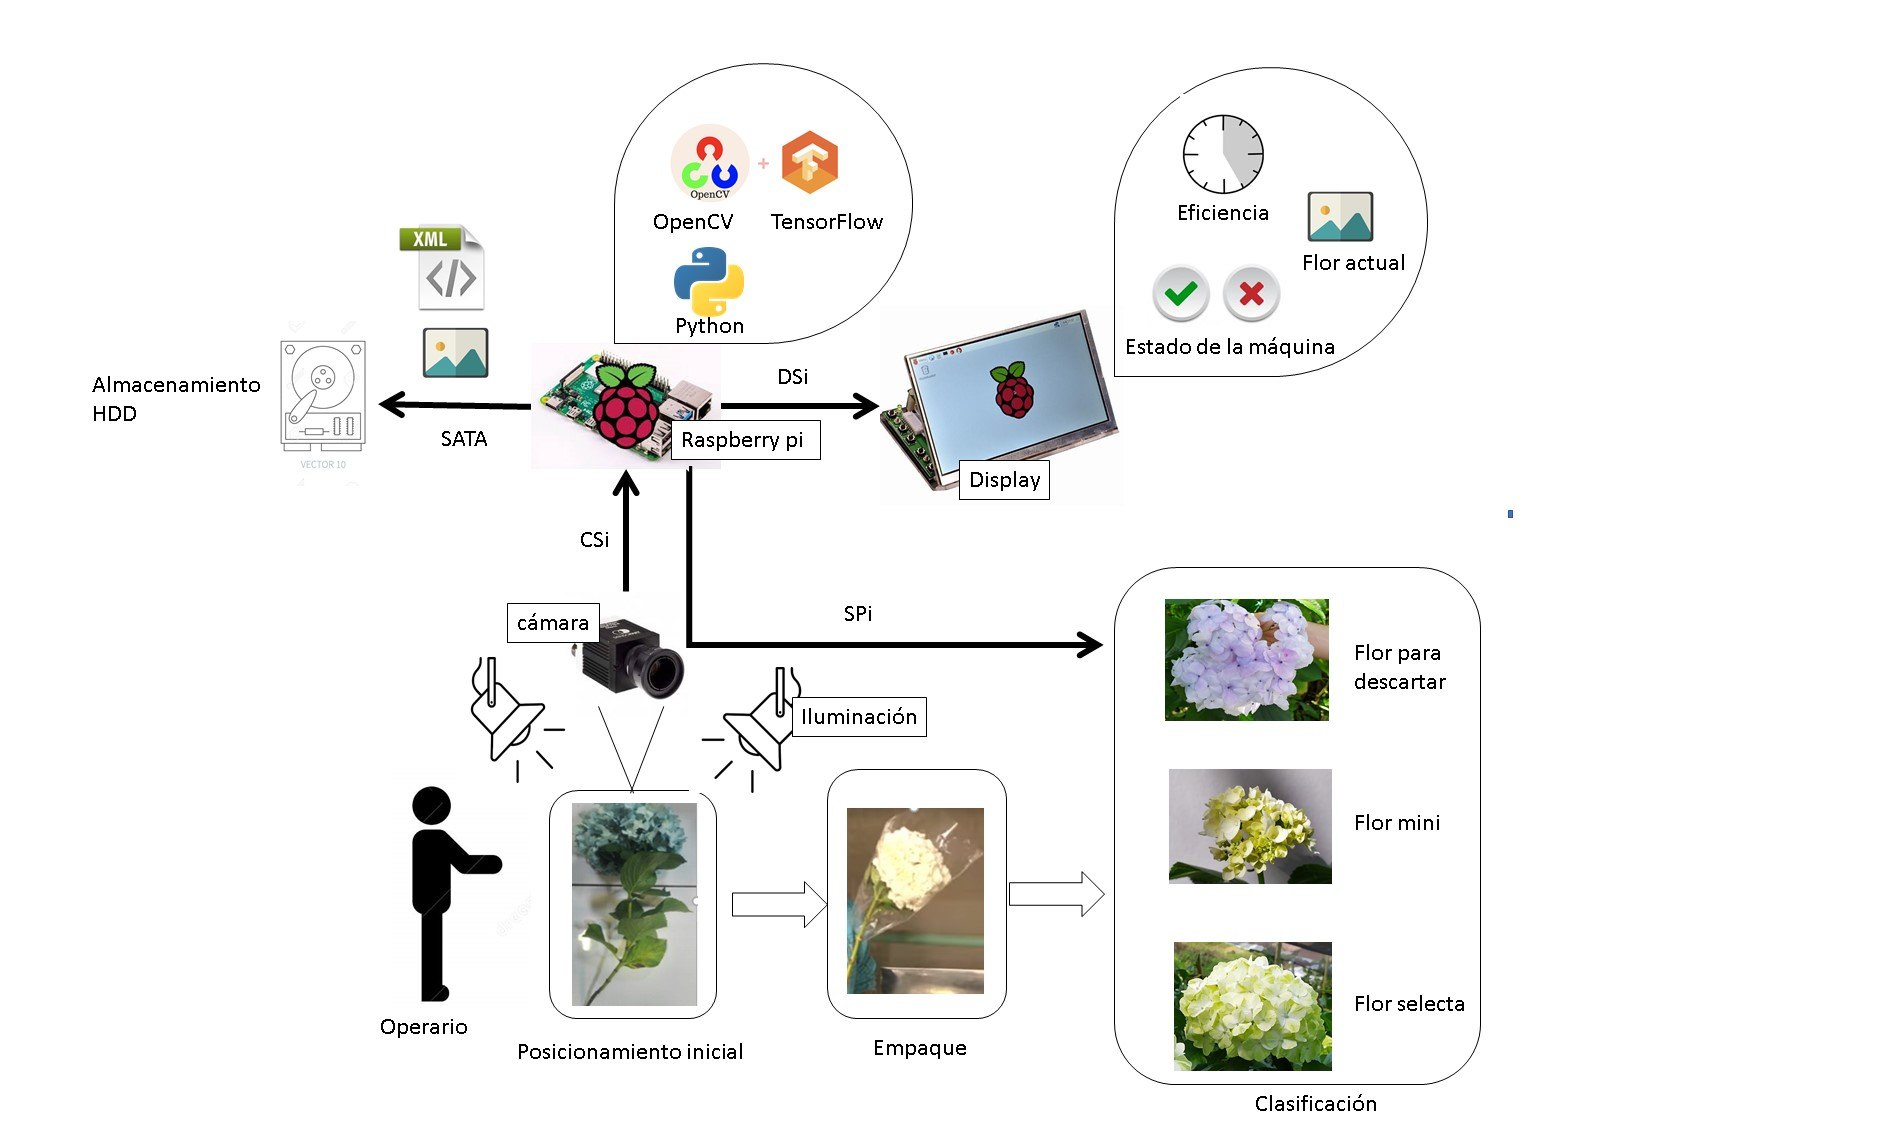
\includegraphics[scale=0.4]{Figuras/Diagrama}
	\caption{Digrama general}
	\label{fig:dGeneral}
\end{figure}


% Table generated by Excel2LaTeX from sheet 'Hoja1'
\begin{table}[H]
	\centering
	\caption{Matriz Necesidades}
	\scalebox{0.9}{
	\begin{tabular}{lp{14.07em}cp{19.855em}p{5.355em}}
		\hline
		\multicolumn{1}{p{2.785em}}{\textbf{\#}} & \textbf{Necesidad} & \multicolumn{1}{p{6em}}{\textbf{Importancia}} & \textbf{Característica} & \textbf{Medida} \\
		\hline
		1  & Reducir tiempos de la postcosecha\newline{} & 5  & Velocidad de operaciones de clasificación empaque y monitoreo & Unidades min \\
		2  & Reducir costo de operación\newline{} & 4  & Costo de postcosecha & COP \\
		3  & Capacidad de los operarios de interactuar con la máquina\newline{} & 3  & Facilidad de operación & Subjetivo \\
		4  & Procesamiento de imágenes\newline{} & 4  & Confiabilidad & \% \\
		5  & Vida Util\newline{} & 3  & Duración del equipo en funcionamiento & Años \\
		\hline
	\end{tabular}}%
	\label{tab:addlabel}%
\end{table}%

Como resultado de la matriz de necesidades se concluye que reducir los tiempos de la postcosecha es el punto más importante solucionar, esto conlleva consigo también una reducción de costos en la operación y que el sistema sea lo suficiente mente confiable para las operaciones que realiza.

\section{Diseño de concepto}
Luego de tener claridad sobre las diferentes necesidades que pretende desarrollar el
proyecto y de haber caracterizado las tareas que realizara la máquina, se procedió a
realizar una diagrama general del sistema, este método permite visualizar el sistema a desarrollar de una
manera sencilla, contemplando únicamente entradas y salidas del sistema.
\begin{figure}[H]
	\centering
	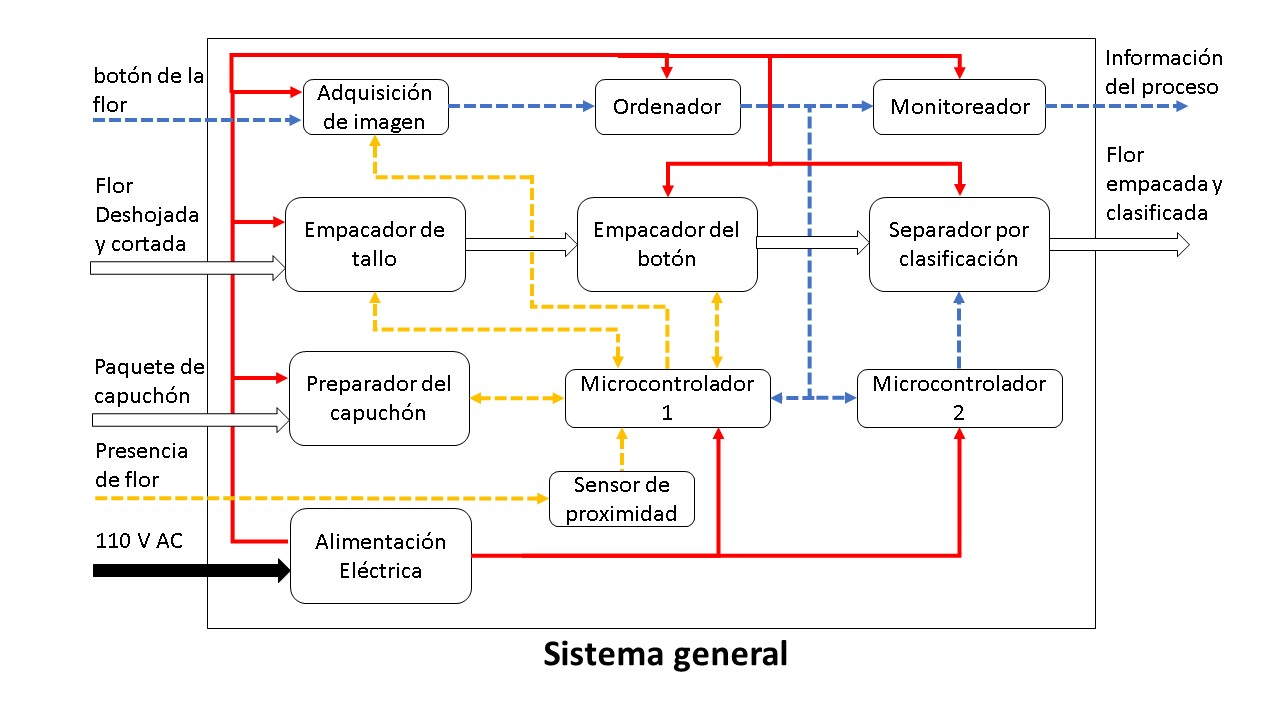
\includegraphics[scale=0.5]{Figuras/SistemaGeneral}
	\caption{Digrama general del sistema}
	\label{fig:dGeneral}
\end{figure}

\subsection{Matriz morfológica}
Para continuar con el diseño de concepto se construye una matriz con las tecnologías
reportadas en cada registro de soluciones, para las diferentes funciones del dispositivo, y
se trazan rutas que definen los componentes que conforman los conceptos preliminares.
\begin{figure}[H]
	\centering
	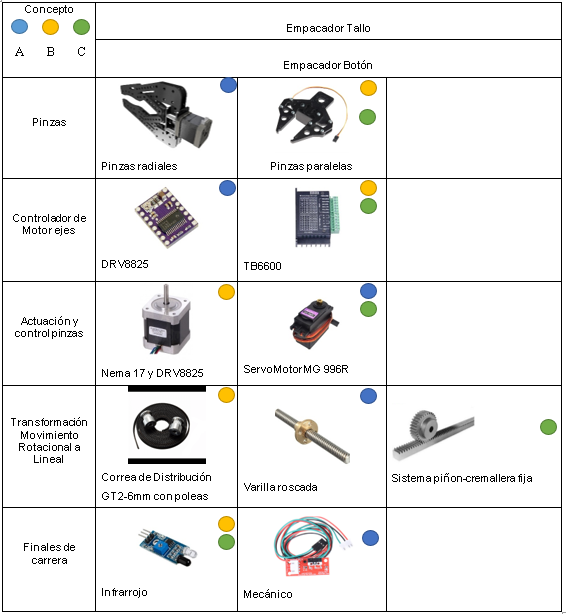
\includegraphics{Figuras/Empacador}
	\caption{Matriz morfologica de subsistemas de empaque tallo y botón}
	\label{fig:MMEmpaque}
\end{figure}
Esta etapas dos etapas se encargan de realizar el empaque de la flor en el capuchón, la primera de ellas el empacador de tallo introduce la flor parcialmente hasta alcanzar el otro extremo del capuchón, donde la segunda etapa el empacador de botón se encarga de finalizar el empacado de la flor introduciendo el botón dentro del capuchón 
\begin{itemize}
	\item \textbf{Concepto A}\\
	Contempla el uso de servo motores, pinzas paralelas, finales de carrera de accionamiento mecánico y un tornillo de bolas para el desplazamiento longitudinal, esta opción es la mejor si se busca suavidad en los movimientos, también requiere poco mantenimiento, pero es la como desventaja tiene que es la más cara, también la integración entre sus componente no es la mejor de las opciones.
	\item \textbf{Concepto B}\\
	Esta opción utiliza motore paso a paso, con pinzas radiales y desplazamiento por medio de una correa de distribución, destaca por su bajo precio, poco mantenimiento y disponibilidad de las piezas, como desventaja tienen que algunas de sus piezas nos son duraderas por lo que se deben cambiar con regularidad
	\item \textbf{Concepto C}\\
	Esta opción es una combinación de las dos anteriores con la diferencia del desplazmiento que se realiza con un piñon cremallera,se caracteriza por su poco mantenimiento y confiabilidad pero su precio es su principal desventaja
\end{itemize}



\begin{figure}[H]
	\centering
	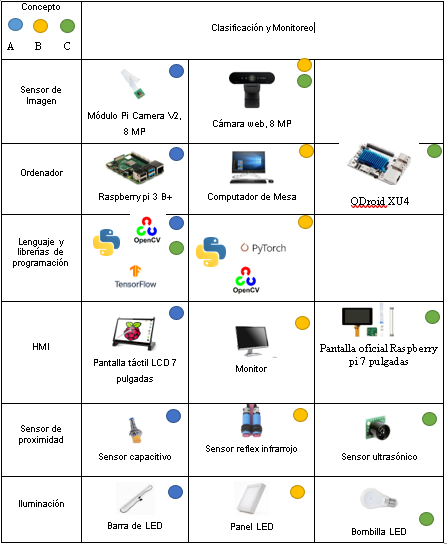
\includegraphics{Figuras/Matriz_Clasificacion}
	\caption{Matriz morfologica de subsistemas de clasificación y monitoreo}
	\label{fig:MMClasificación}
\end{figure}
Esta etapas se hacen cargo de la clasificación y monitoreo de la flor, para realizar utilizan ordenadores camaras y un sistema de iluminación para garantizar 

\begin{itemize}
	\item \textbf{Concepto A}\\
	Esta opcion se caracteriza por su portabilidad y integración entre componentes ya que tanto ordenador, como camara y pantalla son de la plataforma Pi, encuanto a software cuenta como desventaja tiene su limitado poder de procesamiento
	\item \textbf{Concepto B}\\
	Utiliza un ordenador de mesa os cual le otorga  un poder de procesamiento superior a los otros conceptos,como desventaja tiene su baja portabilidad y la calidad de imagenes que puede capturar.
	\item \textbf{Concepto C}\\
	Esta opcion es muy economia debido a su uso de componentes de bajo costo como su ordenador Droid pero tambien la integración entre sus componentes es complicada y la calidad de sus imagenes tambien es inferior a los otros conceptos.
\end{itemize}

\begin{figure}[H]
	\centering
	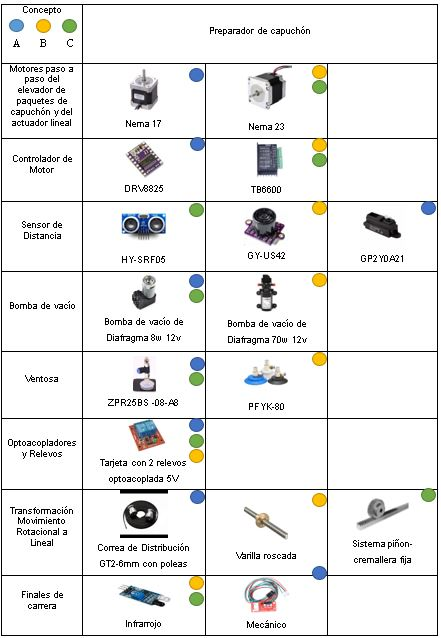
\includegraphics{Figuras/MMCapuchon}
	\caption{Matriz morfologica de subsistema de preparación capuchon}
	\label{fig:MMCapuchon}
\end{figure}
Esta es la primera etapa que controla que microcontrolador 1 y la primera tambíen del ciclo de tareas de todo el sistema. Este subsistema se encarga de preparar/abrir el capuchón en el cúal se insertará posteriormente la flor. Esta función la cumple por medio de un actuador lineal accionado por un motor paso a paso que en su punta posee una ventosa que recibe presión negativa de una bomba de vacío para sujetar un lado del capuchón que finalmente se abre completamente por la fuerza gravitatoria. Estos capuchones son a su vez posicionados para su sujetación a través de un elevador de los paquetes de capuchón que compensa la altura respecto al punto de sujeción a medida que los capuchónes individuales van siendo utilizados, este proceso se efectúa mediante un motor paso a paso que su actuación depende de la altura medida por un sensor de distancia. 
\begin{itemize}
	\item \textbf{Concepto A}\\
	Contempla el uso del motor NEMA 17 para el actuador lineal y del elevador junto con un controlador de corriente pico máxima 2.5 A, un sensor de distancia análogo tipo SHARP con el rango justo para la aplicación, bomba de vacío de 8w, ventosa de fuelle de 25mm, movimiento lineal efectuado por correas de distribución y finales de carrera mecánicos. Esta opción tiene como ventaja más notoria la reducción de precios frente a las otras opciones debido a que se utilizan los elementos más ajustados posibles con elementos comerciales a las especificaciones requeridas pero sacrificando velocidad de actuación debido al motor de menor capacidad. 
	\item \textbf{Concepto B}\\
	Contempla el uso del motor NEMA 23 para el actuador lineal y del elevador junto con un controlador de corriente pico máxima 5 A, un sensor de distancia ultrasónico con rango 20 a 720 cm, bomba de vacío de 8w, ventosa de fuelle de 25mm, movimiento lineal efectuado por Varillas roscadas y finales de carrera reflex infrarojo. Esta opción tiene como ventaja un actuación más rápida respecto a la primera opción, sin embargo, con elementos más costos y con menos precisión en la medición de la altura respecto a la opción anterior, ya que el sensor ultrasónico tiene una resolución de 1cm. 
	\item \textbf{Concepto C}\\
	Contempla el uso del motor NEMA 23 para el actuador lineal y del elevador junto con un controlador de corriente pico máxima 5 A, un sensor de distancia ultrasónico con rango 2 a 450 cm, bomba de vacío de 70w, ventosa de fuelle de 80mm, movimiento lineal efectuado por un sistema piñon-cremallera y finales de carrera reflex infrarojo. Esta opción tiene como ventaja la actuación más rápida respecto a las otras opciones, sin embargo, con los elementos más costos de las opciones en la actuación, además, con la desventaja de que el sistema piñon-cremallera se debería fabricar. En la medición de la altura se contempla uno de los sensores más economicos del mercado y con una resolución de 0.3cm que se encuentra dentro del rango de tolerancia en la medición de distancia. 
\end{itemize}
\begin{figure}[H]
	\centering
	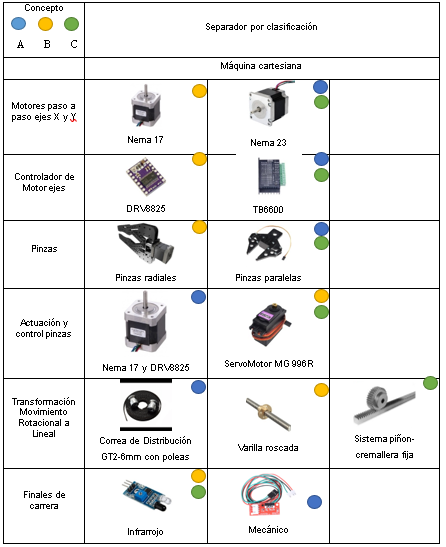
\includegraphics{Figuras/MatrizCartesiana}
	\caption{Matriz morfologica de subsistema de separación por clasificación}
	\label{fig:Cartesiana}
\end{figure}
Esta subsistema la controla el microcontrolador 2 y es la última del ciclo de tareas de todo el sistema. Este subsistema se encarga de clasificar físicamente las flores ingresadas al sistema mediante una máquina cartensiana 2 ejes que sujeta la flor por medio pinzas y las ubica en la base deslizante correspondiente según la clasificación recibida por el ordenador principal.  
\begin{itemize}
	
	\item \textbf{Concepto A}\\
	Contempla el uso del motor NEMA 23 para los dos ejes de movimiento de la máquina cartesiana con movimiento lineal por correas de distribución y poleas. Pinzas paralelas actuadas por un NEMA 17 y su controlador de 2.5 A pico junto con finales de carrera mecánicos. Destaca esta opción por ser la mejor en precio-calidad, con la mayor velocidad de actuación de las opciones consideradas, además del mejor agarre en las pinzas por ser de tipo paralelas y con el NEMA 17. 
	\item \textbf{Concepto B}\\
	Contempla el uso del motor NEMA 17 para los dos ejes de movimiento de la máquina cartesiana con movimiento lineal por varilla roscada. Pinzas radiales actuadas por el ServoMotor MG 996R junto con finales de carrera réflex infrarrojos. Es la opción con menor costo, sin embargo, con una actuación lenta debido a la menor capacidad del motor de los ejes respecto las demás.
	\item \textbf{Concepto C}\\
	Contempla el uso del motor NEMA 23 para los dos ejes de movimiento de la máquina cartesiana con movimiento lineal por un sistema piñon-cremallera. Pinzas paralelas actuadas por el ServoMotor MG 996R junto con finales de carrera réflex infrarrojos. Es una opción con la desventaja de que el sistema piñon-cremallera se debería fabricar, sin embargo, posee una buena velocidad de actuación. 
\end{itemize}

\subsection{Selección de concepto}
Con el objetivo de seleccionar el concepto que permita desarrollar el proyecto de la mejor
manera y obtener los mejores resultados, se utiliza una matriz de decisión, en la que se
especifican diferentes criterios de decisión y su peso, se le da una calificación a cada 
La información presentada en este documento es de exclusiva responsabilidad de los autores y no
compromete a la EIA.
concepto sobre el criterio y se saca un ponderado, al final, el criterio con mayor puntaje en
la suma de los ponderados será el elegido para desarrollar el proyecto.
% Table generated by Excel2LaTeX from sheet 'Hoja1'
\begin{table}[H]
	\centering
	\caption{Matriz de desición Empacador Flor}
	\scalebox{0.9}{
	\begin{tabular}{p{5.355em}cp{5.355em}cp{5.355em}cp{5.355em}c}
		\hline
		\multicolumn{8}{p{42.84em}}{\textbf{Empacador Flor}}
		\\
		\hline
		\multicolumn{2}{c}{} &
		\multicolumn{2}{p{10.71em}}{\textbf{Concepto A}} &
		\multicolumn{2}{p{10.71em}}{\textbf{Concepto B}} &
		\multicolumn{2}{p{10.71em}}{\textbf{Concepto C}}
		\\
		\hline
		\textbf{Criterio de decisión} &
		\multicolumn{1}{p{5.355em}}{\textbf{Peso}} &
		\textbf{C} &
		\multicolumn{1}{p{5.355em}}{\textbf{P}} &
		\textbf{C} &
		\multicolumn{1}{p{5.355em}}{\textbf{P}} &
		\textbf{C} &
		\multicolumn{1}{p{5.355em}}{\textbf{P}}
		\\
		Costos &
		30\% &
	\multicolumn{1}{c}{3} &
		0,9 &
		\multicolumn{1}{c}{4} &
		1,2 &
		\multicolumn{1}{c}{2} &
		0,6
		\\
		Integración entre componentes &
		20\% &
		\multicolumn{1}{c}{4} &
		0,8 &
		\multicolumn{1}{c}{4} &
		0,8 &
		\multicolumn{1}{c}{3} &
		0,6
		\\
		Presición en Posicionamiento &
		10\% &
		\multicolumn{1}{c}{5} &
		0,5 &
		\multicolumn{1}{c}{4} &
		0,4 &
		\multicolumn{1}{c}{3} &
		0,3
		\\
		Suavidad de movimiento &
		5\% &
		\multicolumn{1}{c}{4} &
		0,2 &
		\multicolumn{1}{c}{4} &
		0,2 &
		\multicolumn{1}{c}{3} &
		0,15
		\\
		Disponibilidad &
		15\% &
		\multicolumn{1}{c}{3} &
		0,45 &
		\multicolumn{1}{c}{4} &
		0,6 &
		\multicolumn{1}{c}{3} &
		0,45
		\\
		Facilidad de instalación &
		10\% &
		\multicolumn{1}{c}{3} &
		0,3 &
		\multicolumn{1}{c}{4} &
		0,4 &
		\multicolumn{1}{c}{3} &
		0,3
		\\
		Mantenimiento &
		10\% &
		\multicolumn{1}{c}{3} &
		0,3 &
		\multicolumn{1}{c}{4} &
		0,4 &
		\multicolumn{1}{c}{4} &
		0,4
		\\
		Total &
		&
		\multicolumn{2}{c}{3,45} &
		\multicolumn{2}{c}{4} &
		\multicolumn{2}{c}{2,8}
		\\
		Posición &
		&
		\multicolumn{2}{c}{1} &
		\multicolumn{2}{c}{2} &
		\multicolumn{2}{c}{3}
		\\
		\hline
		\textbf{Desarrollar} &
		&
		\multicolumn{2}{p{10.71em}}{\textbf{SI}} &
		\multicolumn{2}{p{10.71em}}{\textbf{NO}} &
		\multicolumn{2}{p{10.71em}}{\textbf{NO}}
		\\
		\hline
	\end{tabular}}%
	\label{tab:addlabel}%
\end{table}%

% Table generated by Excel2LaTeX from sheet 'Hoja4'
\begin{table}[H]
	\centering
	\caption{Matriz de decisión Clasificador y Monitoreador}
	\scalebox{0.9}{
	\begin{tabular}{p{5.355em}cp{5.355em}cp{5.355em}cp{5.355em}c}
		\hline
		\multicolumn{8}{p{42.84em}}{\textbf{Clasificador y Monitoreador}}
	\\
		\hline
		\multicolumn{2}{c}{} &
		\multicolumn{2}{p{10.71em}}{\textbf{Concepto A}} &
		\multicolumn{2}{p{10.71em}}{\textbf{Concepto B}} &
		\multicolumn{2}{p{10.71em}}{\textbf{Concepto C}}
	\\
		\hline
		\textbf{Criterio de decisión} &
		\multicolumn{1}{p{5.355em}}{\textbf{Peso}} &
		\textbf{C} &
		\multicolumn{1}{p{5.355em}}{\textbf{P}} &
		\textbf{C} &
		\multicolumn{1}{p{5.355em}}{\textbf{P}} &
		\textbf{C} &
		\multicolumn{1}{p{5.355em}}{\textbf{P}}
		\\
		Costos &
		30\% &
		\multicolumn{1}{c}{5} &
		2 &
		\multicolumn{1}{c}{3} &
		1 &
		\multicolumn{1}{c}{4} &
		1,2
		\\
		Integración entre componentes &
		10\% &
		\multicolumn{1}{c}{4} &
		0,4 &
		\multicolumn{1}{c}{4} &
		0,4 &
		\multicolumn{1}{c}{3} &
		0,3
		\\
		Capacidad de procesamiento &
		20\% &
		\multicolumn{1}{c}{3} &
		0,6 &
		\multicolumn{1}{c}{4} &
		0,8 &
		\multicolumn{1}{c}{3} &
		0,6
		\\
		Capacidad de adaptación en clasificación &
		10\% &
		\multicolumn{1}{c}{4} &
		0,4 &
		\multicolumn{1}{c}{4} &
		0,4 &
		\multicolumn{1}{c}{3} &
		0,3
		\\
		Calidad Imágenes &
		10\% &
		\multicolumn{1}{c}{3} &
		0,3 &
		\multicolumn{1}{c}{2} &
		0,2 &
		\multicolumn{1}{c}{2} &
		0,2
		\\
		Disponibilidad &
		10\% &
		\multicolumn{1}{c}{5} &
		0,5 &
		\multicolumn{1}{c}{4} &
		0,4 &
		\multicolumn{1}{c}{3} &
		0,3
		\\
		Facilidad de utilización &
		5\% &
		\multicolumn{1}{c}{4} &
		0,2 &
		\multicolumn{1}{c}{4} &
		0,2 &
		\multicolumn{1}{c}{3} &
		0,15
		\\
		Facilidad de visualización &
		5\% &
		\multicolumn{1}{c}{4} &
		0,2 &
		\multicolumn{1}{c}{4} &
		0,2 &
		\multicolumn{1}{c}{4} &
		0,2
		\\
		Total &
		&
		\multicolumn{1}{c}{4,6} &
		&
		\multicolumn{1}{c}{3,6} &
		&
		\multicolumn{1}{c}{3,25} &
		
		\\
		Posición &
		&
		\multicolumn{1}{c}{1} &
		&
		\multicolumn{1}{c}{2} &
		&
		\multicolumn{1}{c}{3} &
		
		\\
		\hline
		\textbf{Desarrollar} &
		&
		\textbf{SI} &
		&
		\textbf{NO} &
		&
		\textbf{NO} &
		
		\\
		\hline
	\end{tabular}}%
	\label{tab:addlabel}%
\end{table}%

% Table generated by Excel2LaTeX from sheet 'Hoja2'
\begin{table}[H]
	\centering
	\caption{Matriz de decisión Preparador de capuchón}
	\scalebox{0.9}{
	\begin{tabular}{p{5.785em}cp{5.355em}cp{5.355em}cp{5.355em}c}
		\hline
		\multicolumn{8}{p{43.27em}}{\textbf{Preparador de capuchón}}
		\\
		\hline
		\multicolumn{2}{c}{} &
		\multicolumn{2}{p{10.71em}}{\textbf{Concepto A}} &
		\multicolumn{2}{p{10.71em}}{\textbf{Concepto B}} &
		\multicolumn{2}{p{10.71em}}{\textbf{Concepto C}}
		\\
		\hline
		\textbf{Criterio de decisión} &
		\multicolumn{1}{p{5.355em}}{\textbf{Peso}} &
		\textbf{C} &
		\multicolumn{1}{p{5.355em}}{\textbf{P}} &
		\textbf{C} &
		\multicolumn{1}{p{5.355em}}{\textbf{P}} &
		\textbf{C} &
		\multicolumn{1}{p{5.355em}}{\textbf{P}}
		\\
		Costos &
		40\% &
		\multicolumn{1}{c}{5} &
		2 &
		\multicolumn{1}{c}{3} &
		1,2 &
		\multicolumn{1}{c}{2} &
		0,8
		\\
		Integración entre componentes &
		10\% &
		\multicolumn{1}{c}{4} &
		0,4 &
		\multicolumn{1}{c}{4} &
		0,4 &
		\multicolumn{1}{c}{3} &
		0,3
		\\
		Velocidad de actuación &
		30\% &
		\multicolumn{1}{c}{3} &
		0,9 &
		\multicolumn{1}{c}{5} &
		1,5 &
		\multicolumn{1}{c}{5} &
		1,5
		\\
		Disponibilidad &
		10\% &
		\multicolumn{1}{c}{5} &
		0,5 &
		\multicolumn{1}{c}{5} &
		0,5 &
		\multicolumn{1}{c}{3} &
		0,3
		\\
		Facilidad de montaje &
		5\% &
		\multicolumn{1}{c}{4} &
		0,2 &
		\multicolumn{1}{c}{4} &
		0,2 &
		\multicolumn{1}{c}{3} &
		0,15
		\\
		Facilidad de detección de fallas &
		5\% &
		\multicolumn{1}{c}{4} &
		0,2 &
		\multicolumn{1}{c}{3} &
		0,15 &
		\multicolumn{1}{c}{4} &
		0,2
		\\
		Total &
		100\% &
		\multicolumn{2}{c}{4,2} &
		\multicolumn{2}{c}{3,95} &
		\multicolumn{2}{c}{3,25}
		\\
		Posición &
		&
		\multicolumn{2}{c}{1} &
		\multicolumn{2}{c}{2} &
		\multicolumn{2}{c}{3}
		\\
		\hline
		\textbf{Desarrollar} &
		&
		\multicolumn{2}{p{10.71em}}{\textbf{SI}} &
		\multicolumn{2}{p{10.71em}}{\textbf{NO}} &
		\multicolumn{2}{p{10.71em}}{\textbf{NO}}
		\\
		\hline
	\end{tabular}}%
	\label{tab:addlabel}%
\end{table}%

% Table generated by Excel2LaTeX from sheet 'Hoja2'
\begin{table}[H]
	\centering
	\caption{Matriz de desición Separador por clasificación}
	\scalebox{0.9}{
	\begin{tabular}{p{5.785em}cp{5.355em}cp{5.355em}cp{5.355em}c}
		\hline
		\multicolumn{8}{p{43.27em}}{\textbf{Separador por clasificación}}
		\\
		\hline
		\multicolumn{2}{c}{} &
		\multicolumn{2}{p{10.71em}}{\textbf{Concepto A}} &
		\multicolumn{2}{p{10.71em}}{\textbf{Concepto B}} &
		\multicolumn{2}{p{10.71em}}{\textbf{Concepto C}}
		\\
		\hline
		\textbf{Criterio de decisión} &
		\multicolumn{1}{p{5.355em}}{\textbf{Peso}} &
		\textbf{C} &
		\multicolumn{1}{p{5.355em}}{\textbf{P}} &
		\textbf{C} &
		\multicolumn{1}{p{5.355em}}{\textbf{P}} &
		\textbf{C} &
		\multicolumn{1}{p{5.355em}}{\textbf{P}}
		\\
		Costos &
		30\% &
		\multicolumn{1}{c}{4} &
		1,2 &
		\multicolumn{1}{c}{3} &
		0,9 &
		\multicolumn{1}{c}{5} &
		1,5
		\\
		Integración entre componentes &
		10\% &
		\multicolumn{1}{c}{4} &
		0,4 &
		\multicolumn{1}{c}{4} &
		0,4 &
		\multicolumn{1}{c}{3} &
		0,3
		\\
		Velocidad de actuación &
		40\% &
		\multicolumn{1}{c}{5} &
		2 &
		\multicolumn{1}{c}{3} &
		1,2 &
		\multicolumn{1}{c}{4} &
		1,6
		\\
		Disponibilidad &
		10\% &
		\multicolumn{1}{c}{5} &
		0,5 &
		\multicolumn{1}{c}{5} &
		0,5 &
		\multicolumn{1}{c}{3} &
		0,3
		\\
		Facilidad de montaje &
		5\% &
		\multicolumn{1}{c}{4} &
		0,2 &
		\multicolumn{1}{c}{4} &
		0,2 &
		\multicolumn{1}{c}{3} &
		0,15
		\\
		Facilidad de detección de fallas &
		5\% &
		\multicolumn{1}{c}{4} &
		0,2 &
		\multicolumn{1}{c}{3} &
		0,15 &
		\multicolumn{1}{c}{3} &
		0,15
		\\
		Total &
		100\% &
		\multicolumn{2}{c}{4,5} &
		\multicolumn{2}{c}{3,35} &
		\multicolumn{2}{c}{4}
		\\
		Posición &
		&
		\multicolumn{2}{c}{1} &
		\multicolumn{2}{c}{2} &
		\multicolumn{2}{c}{3}
		\\
		\hline
		\textbf{Desarrollar} &
		&
		\multicolumn{2}{p{10.71em}}{\textbf{SI}} &
		\multicolumn{2}{p{10.71em}}{\textbf{NO}} &
		\multicolumn{2}{p{10.71em}}{\textbf{NO}}
		\\
		\hline
	\end{tabular}}%
	\label{tab:addlabel}%
\end{table}%



\section{Diagrama de bloques del sistema}
Los diagramas de bloques del sistema permiten ver en profundidad la interacción de cada uno de los componentes, realizar este diagrama permite evaluar los conceptos seleccionados por que en este se observan las integraciones entre componentes por lo que es muy sencillo observar posibles fallos de la solución y dimensionar los componentes a obtener.
\begin{figure}[H]
	\centering
	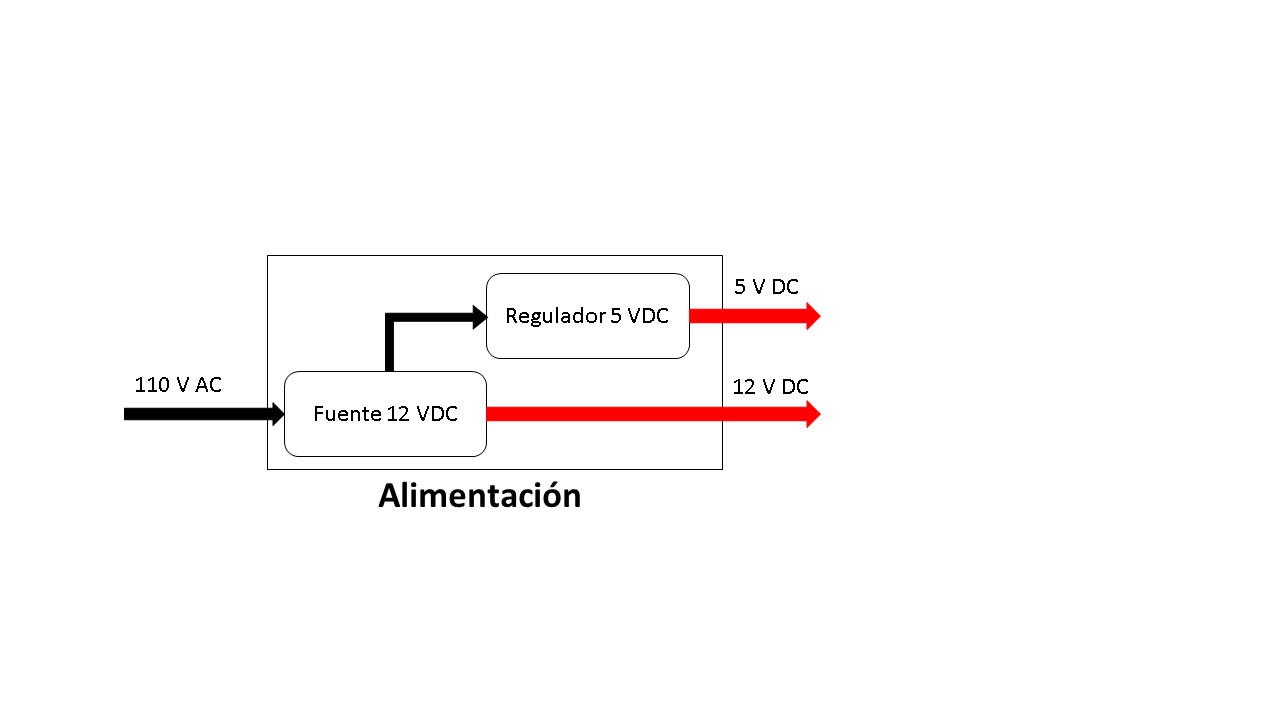
\includegraphics[scale=0.4]{Figuras/Alimentacion}
	\caption{Diagrama de bloques alimentación}
	\label{fig:DBAlimentacion}
\end{figure}

\begin{figure}[htb]
	\centering
	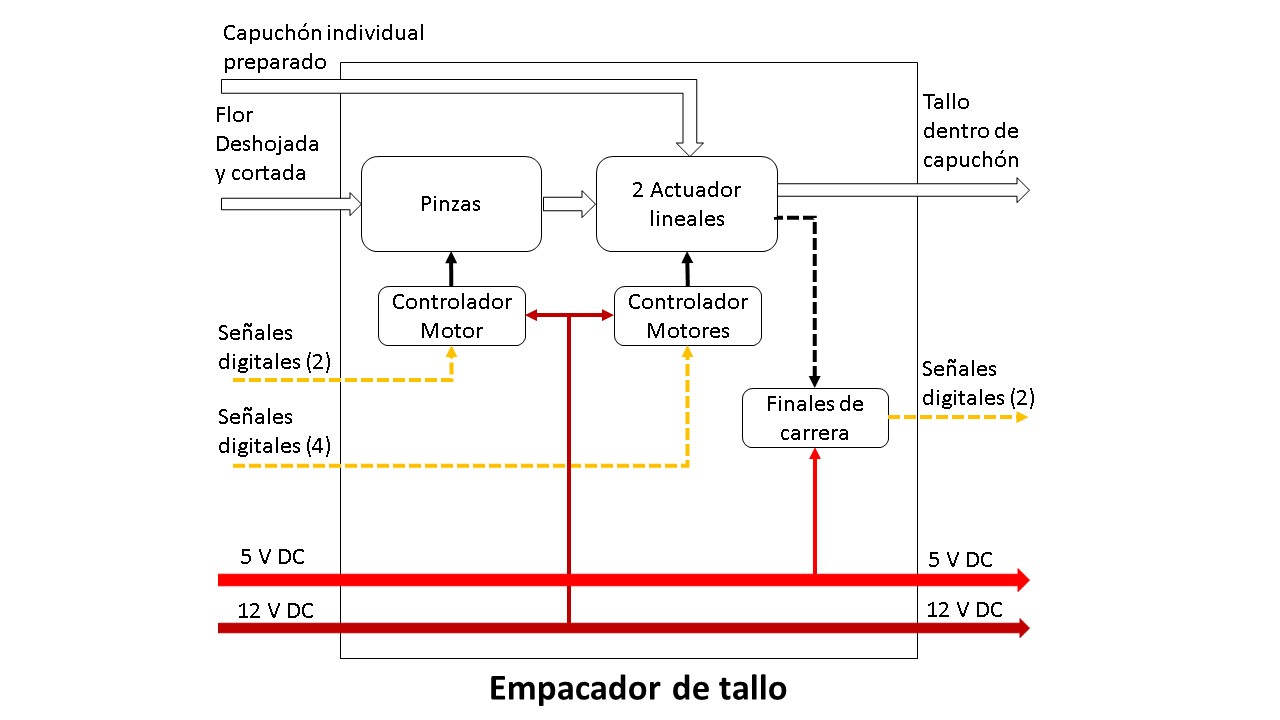
\includegraphics[scale=0.4]{Figuras/PreparadorTallo}
	\caption{Diagrama de bloques empacador de tallo}
	\label{fig:DBAlimentacion}
\end{figure}
\begin{figure}[H]
	\centering
	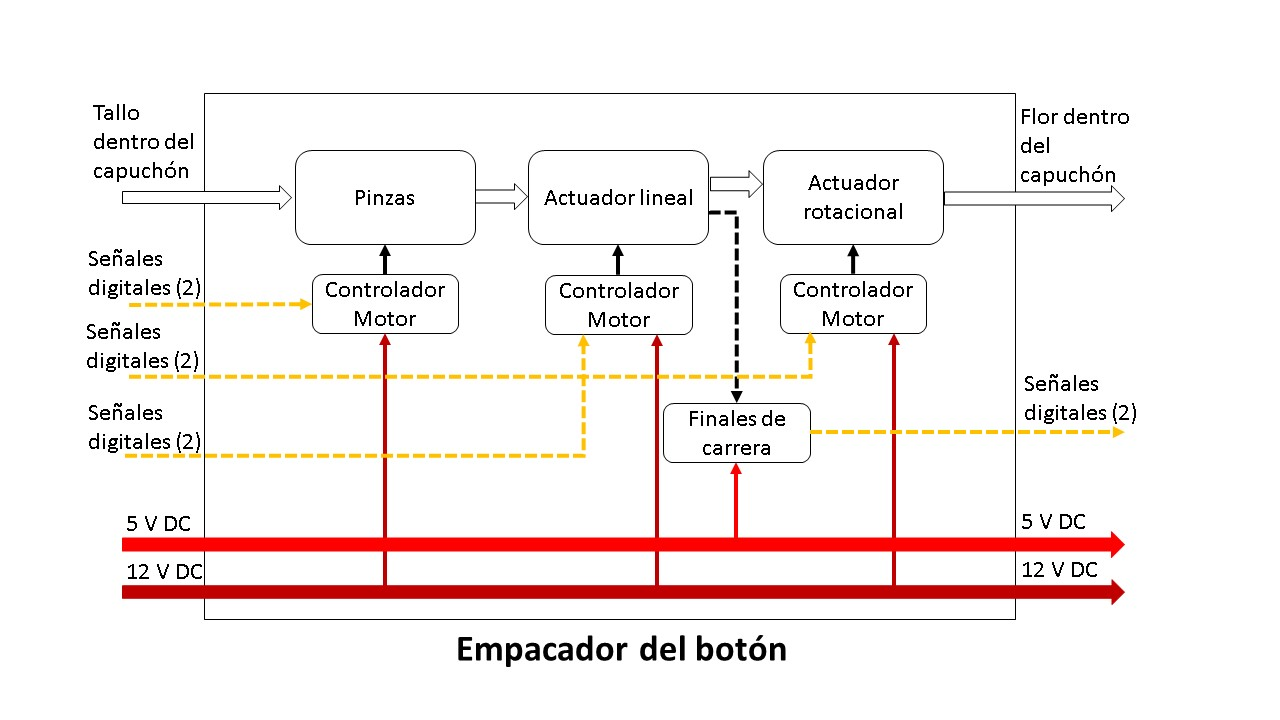
\includegraphics[scale=0.4]{Figuras/EmpacadorBoton}
	\caption{Diagrama de bloques empacador botón}
	\label{fig:DBAlimentacion}
\end{figure}
\begin{figure}[H]
	\centering
	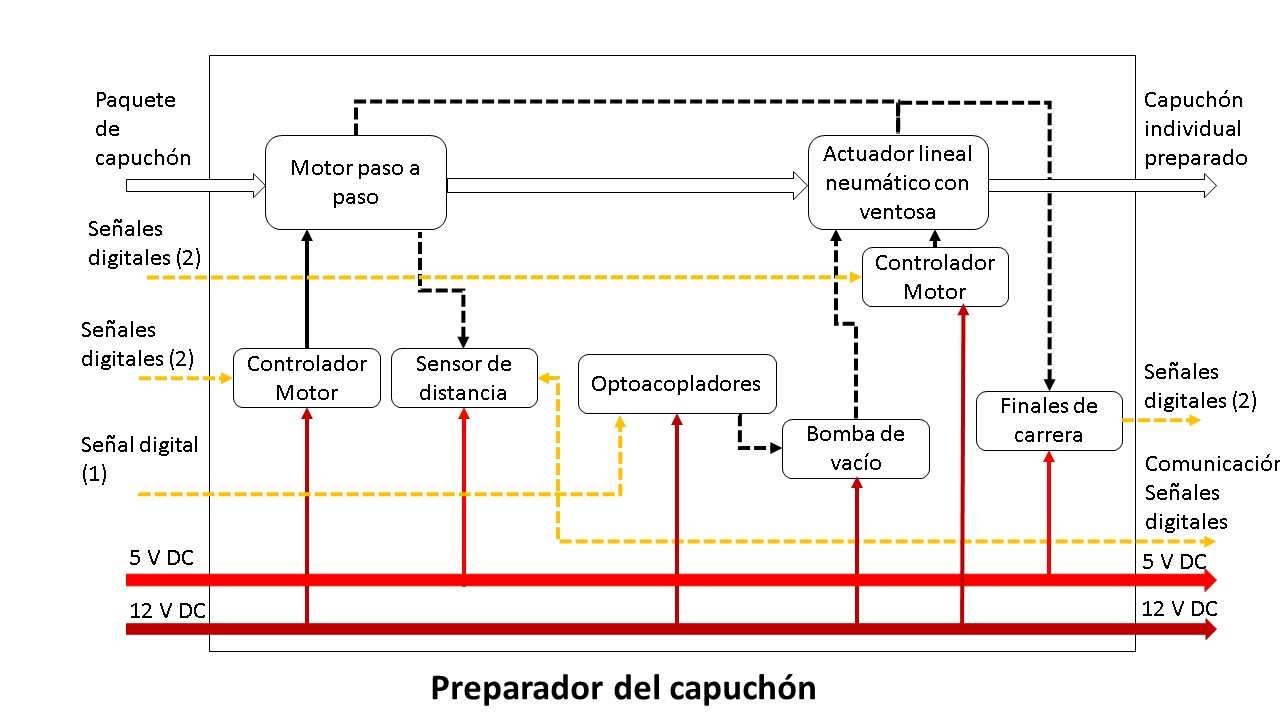
\includegraphics[scale=0.5]{Figuras/PreparadorCapuchon}
	\caption{Diagrama de bloques preparador capuchón}
	\label{fig:DBAlimentacion}
\end{figure}


\begin{figure}[H]
	\centering
	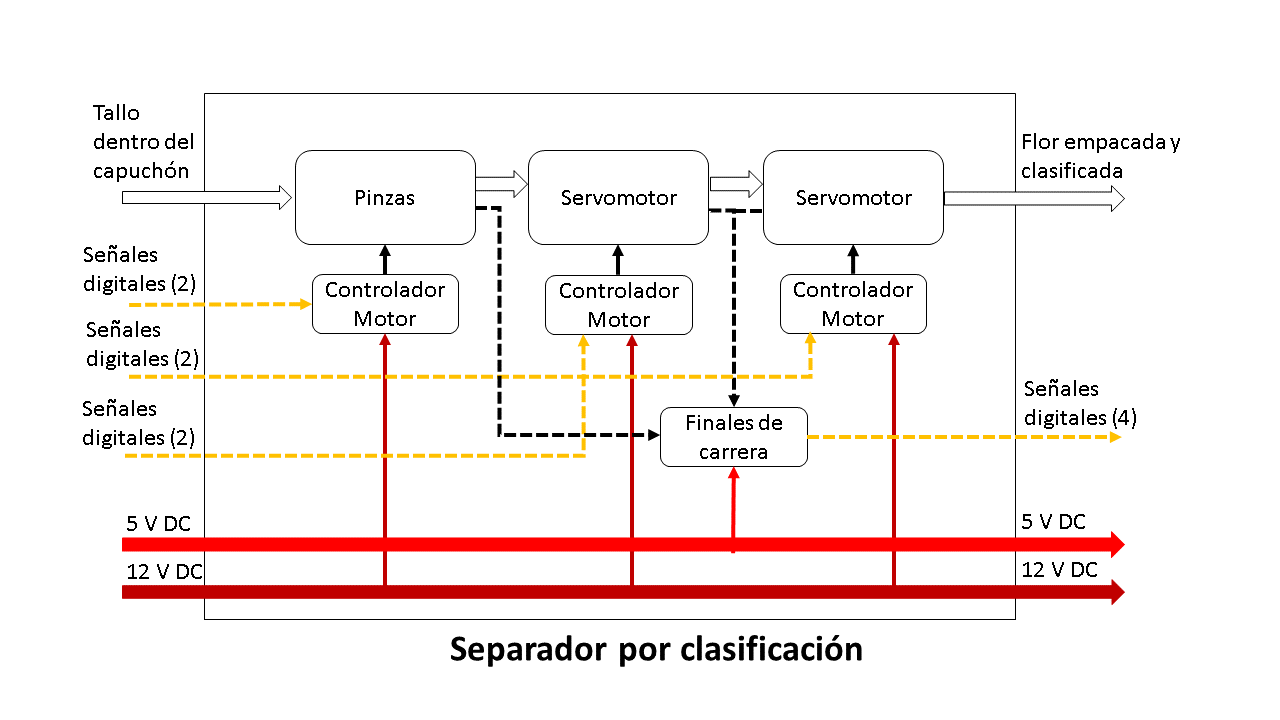
\includegraphics[scale=0.4]{Figuras/SeparadorClasificacion}
	\caption{Diagrama de bloques alimentación}
	\label{fig:DBAlimentacion}
\end{figure}

\begin{figure}[H]
	\centering
	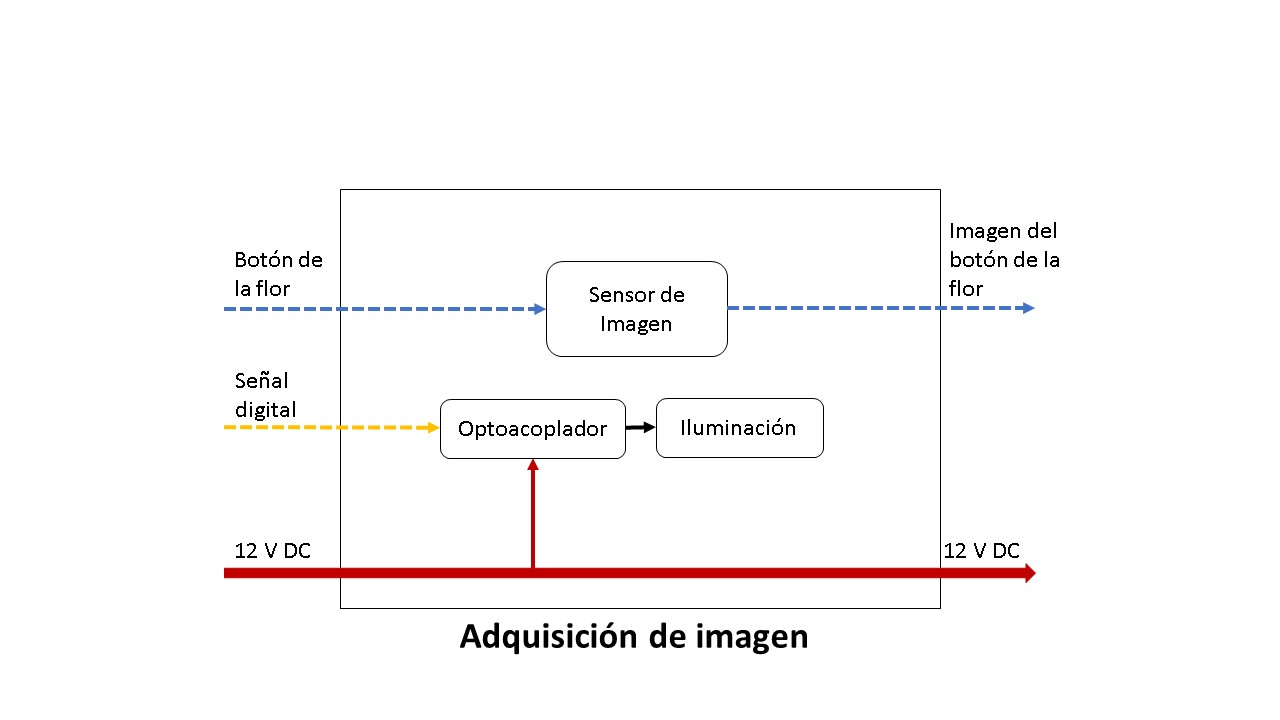
\includegraphics[scale=0.4]{Figuras/AdquisicionImagen}
	\caption{Diagrama de bloques alimentación}
	\label{fig:DBAlimentacion}
\end{figure}

\begin{figure}[H]
	\centering
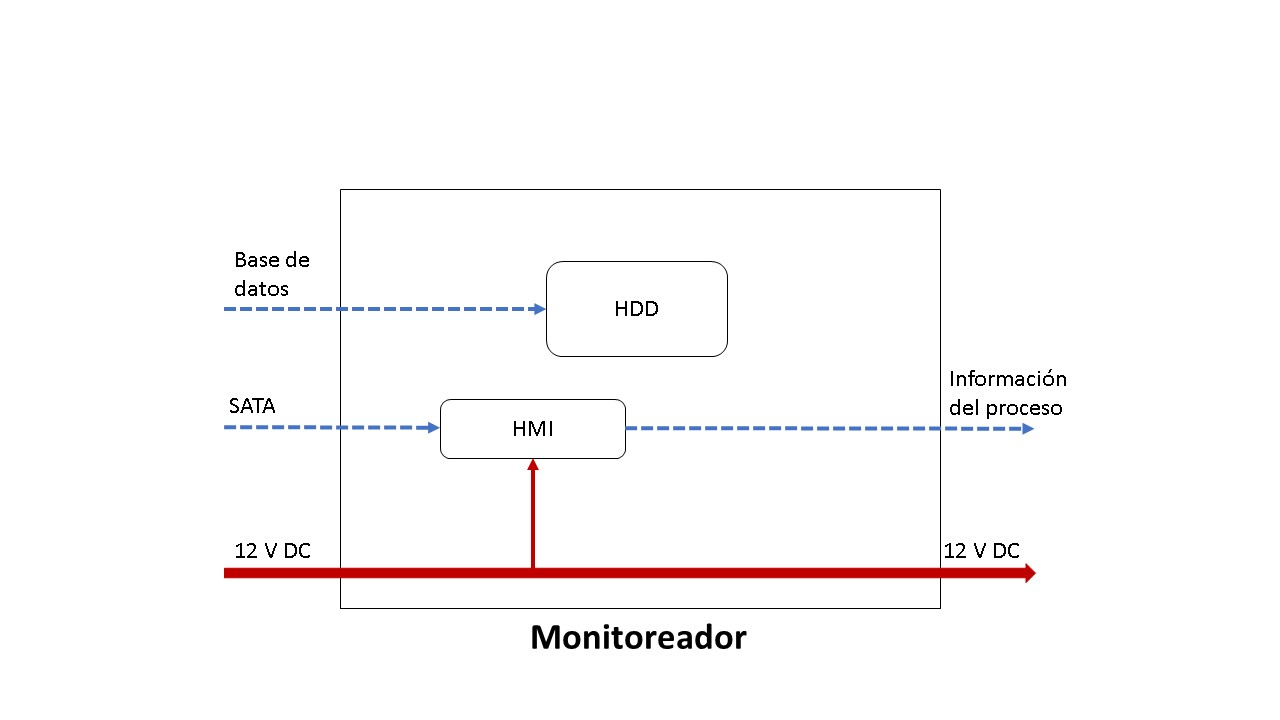
\includegraphics[scale=0.4]{Figuras/Monitoreador}
	\caption{Diagrama de bloques alimentación}
	\label{fig:DBAlimentacion}
\end{figure}

\chapterend{}

%\part{Resultados}

% Resultados ejecucion proyecto

%%%%%%%%%%%%%%%%%%%%%%%%%%%%%%%%%%%%%%%%%%%%%%%%%%%%%%%%%%%%%%%%%%%
%%% Documento LaTeX 											%%%
%%%%%%%%%%%%%%%%%%%%%%%%%%%%%%%%%%%%%%%%%%%%%%%%%%%%%%%%%%%%%%%%%%%
% Título:	Plantilla de TFG/TFM
% Autor:  Carlos Andres Goez, Juan Pablo Baena 
% Fecha:  2020-03-12
%%%%%%%%%%%%%%%%%%%%%%%%%%%%%%%%%%%%%%%%%%%%%%%%%%%%%%%%%%%%%%%%%%%
%	Modo:					PDFLaTeX.
%%%%%%%%%%%%%%%%%%%%%%%%%%%%%%%%%%%%%%%%%%%%%%%%%%%%%%%%%%%%%%%%%%%
%------------------------------
\chapterbegin{Título del capítulo}
\label{chp:Utiliz}
\minitoc

\section{Título de la sección}
\label{sec:TestSuiteCrec}

\section{Título de la sección}

\chapterend{}

%\part{Conclusiones}

% Conclusiones del proyecto

%%%%%%%%%%%%%%%%%%%%%%%%%%%%%%%%%%%%%%%%%%%%%%%%%%%%%%%%%%%%%%%%%%%
%%% Documento LaTeX 											%%%
%%%%%%%%%%%%%%%%%%%%%%%%%%%%%%%%%%%%%%%%%%%%%%%%%%%%%%%%%%%%%%%%%%%
% Título:	Plantilla de TFG/TFM
% Autor:  Carlos Andres Goez, Juan Pablo Baena 
% Fecha:  2020-03-12
%%%%%%%%%%%%%%%%%%%%%%%%%%%%%%%%%%%%%%%%%%%%%%%%%%%%%%%%%%%%%%%%%%%
%	Modo:					PDFLaTeX.
%%%%%%%%%%%%%%%%%%%%%%%%%%%%%%%%%%%%%%%%%%%%%%%%%%%%%%%%%%%%%%%%%%%
%------------------------------


\chapterbeginx{Conclusiones y líneas futuras}

Después de todo el desarrollo del proyecto, es pertinente hacer una
valoración final del mismo, respecto a los resultados obtenidos, las
expectativas o el resultado de la experiencia acumulada.

Esta sección es indispensable y en ella se ha de reflejar, lo más
claramente posible, las aportaciones del trabajo con unas conclusiones
finales.

Además, considerando también el estado de la técnica, se deben indicar
las posibles líneas futuras de trabajo, proponer otros puntos de vista
o cualquier otra sugerencia como postámbulo del presente trabajo, para
ser considerada por el lector o el tribunal evaluador.


\chapterend

\appendix

%%%%%%%%%%%%%%%%%%%%%%%%%%%%%%%%%%%%%%%%%%%%%%%%%%%%%%%%%%%%%%%%%%%
%%% Documento LaTeX 											%%%
%%%%%%%%%%%%%%%%%%%%%%%%%%%%%%%%%%%%%%%%%%%%%%%%%%%%%%%%%%%%%%%%%%%
% Título:	Plantilla de TFG/TFM
% Autor:  Carlos Andres Goez, Juan Pablo Baena 
% Fecha:  2020-03-12
%%%%%%%%%%%%%%%%%%%%%%%%%%%%%%%%%%%%%%%%%%%%%%%%%%%%%%%%%%%%%%%%%%%
%	Modo:					PDFLaTeX.
%%%%%%%%%%%%%%%%%%%%%%%%%%%%%%%%%%%%%%%%%%%%%%%%%%%%%%%%%%%%%%%%%%%
%------------------------------


\chapterbeginx{ANEXO 1}




\chapterend
% Formato de documento en la parte final.
\backmatter
%Hace que los capítulos y títulos nivel inferior no aparezcan numerados (lo que es ideal para conclusiones o notas finales).

% Bibliografía


%%%%%%%%%%%%%%%%%%%%%%%%%%%%%%%%%%%%%%%%%%%%%%%%%%%%%%%%%%%%%%%%%%%
%%% Documento LaTeX 											%%%
%%%%%%%%%%%%%%%%%%%%%%%%%%%%%%%%%%%%%%%%%%%%%%%%%%%%%%%%%%%%%%%%%%%
% Título:	Plantilla de TFG/TFM
% Autor:  Carlos Andres Goez, Juan Pablo Baena 
% Fecha:  2020-03-12
%%%%%%%%%%%%%%%%%%%%%%%%%%%%%%%%%%%%%%%%%%%%%%%%%%%%%%%%%%%%%%%%%%%
%	Modo:					PDFLaTeX.
%%%%%%%%%%%%%%%%%%%%%%%%%%%%%%%%%%%%%%%%%%%%%%%%%%%%%%%%%%%%%%%%%%%
%------------------------------
% Encabezamiento %
\pagestyle{fancy}
\fancyhead[LE,RO]{\thepage}
\fancyhead[RE,LO]{Bibliografía}

%Inclusión de bibliografía%
\bibliography{Bibliografia} %Úsese el nombre del fichero sin extensión

%Inclusión en el índice (Tabla de contenidos)
\addcontentsline{toc}{chapter}{Bibliografía}

%Formateo de estilo de bibliografía
% Otros formatos: plain, unsrt, abbrv
%  plain: las entradas se ordenan alfabéticamente y se etiquetan con un número (p.ej., [1])
% unsrt: igual que plain, pero aparecen en orden de citación.
% alpha: el etiquetado se hace por autor y año de publicación (p.ej., [Knu66]).
% abbrv: igual que alpha, pero más abreviado.
\bibliographystyle{plain}

%Impresión de todas las entradas bibliográficas aunque no estén citadas
%\nocite{*}

\chapterend

	
\end{document}

